%%%%%%%%%%%%%%%%%%%%%%%%%%%%%%%%%%%%%%%%%%%%%%%%%%%%%%%%%%%%%%%%%%%%%
% LaTeX Template: Softwaretechnik SS 2017
%
% Date: April 2017
%
%%%%%%%%%%%%%%%%%%%%%%%%%%%%%%%%%%%%%%%%%%%%%%%%%%%%%%%%%%%%%%%%%%%%%%

\documentclass[12pt]{article}
\usepackage[a4paper]{geometry}
\usepackage{framed}
\usepackage[myheadings]{fullpage}
\usepackage{fancyhdr}
\usepackage{lastpage}
\usepackage{graphicx, wrapfig, subcaption, setspace, booktabs}
% \usepackage{movie15}
\usepackage[T1]{fontenc}
\usepackage[font=small, labelfont=bf]{caption}
\usepackage[protrusion=true, expansion=true]{microtype}
\usepackage[german]{babel}
\usepackage{sectsty}
\usepackage{url, lipsum}
\usepackage[parfill]{parskip}


%-------------------------------------------------------------------------------
% Commands
%-------------------------------------------------------------------------------
\newcommand{\HRule}[1]{\rule{\linewidth}{#1}}
\input{../env}
%-------------------------------------------------------------------------------
% HEADER & FOOTER
%-------------------------------------------------------------------------------
\pagestyle{fancy}
\fancyhf{}
\setlength\headheight{15pt}
\fancyhead[L]{\newCommandName}
\fancyhead[R]{\newCommandUniversity}
\fancyfoot[R]{Seite \thepage\ von \pageref{LastPage}}

%-------------------------------------------------------------------------------
% TITLE PAGE
%-------------------------------------------------------------------------------
\begin{document}


\title{ \normalsize
		\HRule{0.5pt} \\
		\LARGE \textbf{\uppercase{\newCommandDiscipline}} \\
    \smallbreak
		\small\textbf{{\newCommandTerm}}\\
		\HRule{2pt} \\ [0.5cm]
		\normalsize \today \vspace*{10\baselineskip}}

\date{}

\author{
		\newCommandName \\
		\newCommandMatriculationNumber \\
		\newCommandUniversity \\
		\newCommandFaculty
}

\pagenumbering{gobble}

\maketitle

\newpage

\pagenumbering{arabic}


%-------------------------------------------------------------------------------
% Section title formatting
\sectionfont{\scshape}
%-------------------------------------------------------------------------------

%-------------------------------------------------------------------------------
% BODY
%-------------------------------------------------------------------------------

\section{SWT - Einf"uhrung in die Softwaretechnik}

%-------------------------------------------------------------------------------
% #1
%-------------------------------------------------------------------------------
\subsection{"Ubung SWT-01}
\subsubsection*{Aufgabe:}

\begin{framed}
\textbf{Softwaretechnik allgemein}
\smallbreak
Was ist Softwaretechnik? Was wird da gelehrt? Worum geht es?
\\
Was antworten Sie?
\bigbreak
\small Bearbeitungszeit: 10 Minuten
\end{framed}
\bigbreak
\bigbreak
\subsubsection*{L"osung:}
Lorem ipsum dolor sit amet, consectetur adipisicing elit, sed do eiusmod tempor incididunt ut labore et dolore magna aliqua. Ut enim ad minim veniam, quis nostrud exercitation ullamco laboris nisi ut aliquip ex ea commodo consequat. Duis aute irure dolor in reprehenderit in voluptate velit esse cillum dolore eu fugiat nulla pariatur. Excepteur sint occaecat cupidatat non proident, sunt in culpa qui officia deserunt mollit anim id est laborum.
Lorem ipsum dolor sit amet, consectetur adipisicing elit, sed do eiusmod tempor incididunt ut labore et dolore magna aliqua. Ut enim ad minim veniam, quis nostrud exercitation ullamco laboris nisi ut aliquip ex ea commodo consequat. Duis aute irure dolor in reprehenderit in voluptate velit esse cillum dolore eu fugiat nulla pariatur. Excepteur sint occaecat cupidatat non proident, sunt in culpa qui officia deserunt mollit anim id est laborum.

%-------------------------------------------------------------------------------
% #2
%-------------------------------------------------------------------------------
\newpage
\subsection{"Ubung SWT-02}
\subsubsection*{Aufgabe:}

\begin{framed}
\textbf{Softwarelebenszyklus}
\smallbreak
Sie werden in einem Bewerbungsgespr"ach gebeten, die wesentlichen Teile des Softwarelebenszyklus an dem Whiteboard zu skizzieren und zu erl"autern.
\\ K"onnen Sie das?
\bigbreak
\small Bearbeitungszeit: 15 Minuten
\end{framed}
\bigbreak
\bigbreak
\subsubsection*{L"osung:}
Lorem ipsum dolor sit amet, consectetur adipisicing elit, sed do eiusmod tempor incididunt ut labore et dolore magna aliqua. Ut enim ad minim veniam, quis nostrud exercitation ullamco laboris nisi ut aliquip ex ea commodo consequat. Duis aute irure dolor in reprehenderit in voluptate velit esse cillum dolore eu fugiat nulla pariatur. Excepteur sint occaecat cupidatat non proident, sunt in culpa qui officia deserunt mollit anim id est laborum.

%-------------------------------------------------------------------------------
% #3
%-------------------------------------------------------------------------------
\newpage
\subsection{"Ubung SWT-03}
\subsubsection*{Aufgabe:}

\begin{framed}
\textbf{Prinzipien}
\smallbreak
Geben Sie bitte zu jedem Prinzip der Softwaretechnik (Abstraktion, Strukturierung, Hierarchisierung, Modularisierung, Standardisierung) ein Beispiel an. Wo ist Ihnen das schon begegnet und wo k"onnte das in der Softwaretechnik angewendet oder wirksam werden?
\bigbreak
\small Bearbeitungszeit: 10 Minuten
\end{framed}
\bigbreak
\bigbreak
\subsubsection*{L"osung:}
Lorem ipsum dolor sit amet, consectetur adipisicing elit, sed do eiusmod tempor incididunt ut labore et dolore magna aliqua. Ut enim ad minim veniam, quis nostrud exercitation ullamco laboris nisi ut aliquip ex ea commodo consequat. Duis aute irure dolor in reprehenderit in voluptate velit esse cillum dolore eu fugiat nulla pariatur. Excepteur sint occaecat cupidatat non proident, sunt in culpa qui officia deserunt mollit anim id est laborum.

%-------------------------------------------------------------------------------
% #4
%-------------------------------------------------------------------------------
\newpage
\subsection{"Ubung SWT-04}
\subsubsection*{Aufgabe:}

\begin{framed}
\textbf{Recherche}
\smallbreak
Recherchieren Sie bitte im Internet "uber Softwaretechnik oder Softwareengineering. Welche Bereiche interessieren Sie ganz besonders?
\bigbreak
\small Bearbeitungszeit: 30 Minuten
\end{framed}
\bigbreak
\bigbreak
\subsubsection*{L"osung:}
Lorem ipsum dolor sit amet, consectetur adipisicing elit, sed do eiusmod tempor incididunt ut labore et dolore magna aliqua. Ut enim ad minim veniam, quis nostrud exercitation ullamco laboris nisi ut aliquip ex ea commodo consequat. Duis aute irure dolor in reprehenderit in voluptate velit esse cillum dolore eu fugiat nulla pariatur. Excepteur sint occaecat cupidatat non proident, sunt in culpa qui officia deserunt mollit anim id est laborum.

%-------------------------------------------------------------------------------
% #5
%-------------------------------------------------------------------------------
\newpage
\subsection{"Ubung SWT-05}
\subsubsection*{Aufgabe:}

\begin{framed}
\textbf{Wissensfragen zur Lerneinheit}
\smallbreak
Versuchen Sie die Fragen schriftlich zu beantworten ohne noch einmal in der Lerneinheit nachzuschlagen.
\begin{enumerate}
\item An welche Best Practices erinnern Sie sich oder welche haben Sie verinnerlicht?
\item Warum ist es sinnvoll Softwarefehler fr"uh zu erkennen?
\item Was geht in Softwareprojekten typischerweise schief?
\item Kennen Sie (Standardisierungs-)Organisationen, die sich mit Software besch"aftigen?
\end{enumerate}
\bigbreak
\small Bearbeitungszeit: 15 Minuten
\end{framed}
\bigbreak
\bigbreak
\subsubsection*{L"osung:}
Lorem ipsum dolor sit amet, consectetur adipisicing elit, sed do eiusmod tempor incididunt ut labore et dolore magna aliqua. Ut enim ad minim veniam, quis nostrud exercitation ullamco laboris nisi ut aliquip ex ea commodo consequat. Duis aute irure dolor in reprehenderit in voluptate velit esse cillum dolore eu fugiat nulla pariatur. Excepteur sint occaecat cupidatat non proident, sunt in culpa qui officia deserunt mollit anim id est laborum.

%-------------------------------------------------------------------------------
% #6
%-------------------------------------------------------------------------------
\newpage
\subsection{"Ubung SWT-06}
\subsubsection*{Aufgabe:}

\begin{framed}
\textbf{Fehlerquellen}
\smallbreak
H"aufige Fehlerquellen in Softwareprojekten sind:
\bigbreak
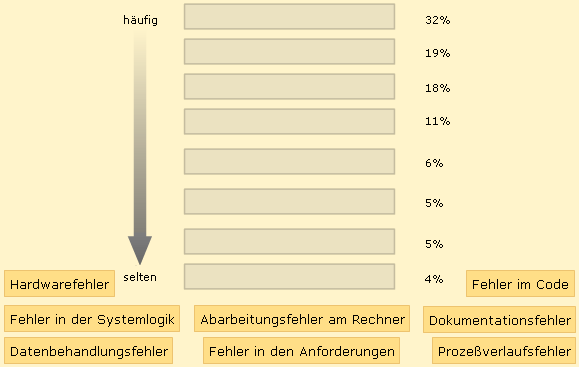
\includegraphics[width=1.0\textwidth]{./images/ueb01-06.png}
\end{framed}
\bigbreak
\bigbreak
\subsubsection*{L"osung:}
Lorem ipsum dolor sit amet, consectetur adipisicing elit, sed do eiusmod tempor incididunt ut labore et dolore magna aliqua. Ut enim ad minim veniam, quis nostrud exercitation ullamco laboris nisi ut aliquip ex ea commodo consequat. Duis aute irure dolor in reprehenderit in voluptate velit esse cillum dolore eu fugiat nulla pariatur. Excepteur sint occaecat cupidatat non proident, sunt in culpa qui officia deserunt mollit anim id est laborum.

%-------------------------------------------------------------------------------
% #7
%-------------------------------------------------------------------------------
\newpage
\subsection{"Ubung SWT-07}
\subsubsection*{Aufgabe:}

\begin{framed}
\textbf{Phaseneinteilung}
\smallbreak
Ordnen Sie die Phasen und Ergebnisse des Softwarelebenszyklus in der richtigen Reihenfolge an.
\bigbreak
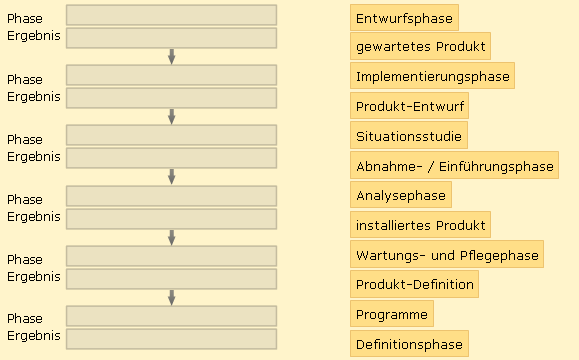
\includegraphics[width=1.0\textwidth]{./images/ueb01-07.png}
\end{framed}
\bigbreak
\bigbreak
\subsubsection*{L"osung:}
Lorem ipsum dolor sit amet, consectetur adipisicing elit, sed do eiusmod tempor incididunt ut labore et dolore magna aliqua. Ut enim ad minim veniam, quis nostrud exercitation ullamco laboris nisi ut aliquip ex ea commodo consequat. Duis aute irure dolor in reprehenderit in voluptate velit esse cillum dolore eu fugiat nulla pariatur. Excepteur sint occaecat cupidatat non proident, sunt in culpa qui officia deserunt mollit anim id est laborum.









%-------------------------------------------------------------------------------
% ENDE
%-------------------------------------------------------------------------------

\end{document}
